

\section{Welcome to YAMS!}

YAMS is a simulator for the MIPS processor, which runs a RISC (Reduced Instruction Set Chip) architecture.  As a simulator, it's main task is to correctly simulate a given set of assembler instructions and produce any necessary output.  In addition, there are many features that let you see exactly what is happening as each instruction is executed, such as register and memory contents.  YAMS also includes a comprehensive statistics module so you can see just how efficient the assmebly code is.

The YAMS package will work in two formats - in a console that will run from a command line, and in a user friendly graphical version, so you can see clearly what is happening inside the processor as the assmebly program is being executed.

\section{Requirements For All Versions of YAMS}

YAMS is written in Java. Hence it requires a JRE (Java Runtime Environment) to run.

If you are unsure if you have one, type in console and fingers crossed:

\texttt{\$ java -version}

If you don't get something like \texttt{Command not found}, YAMS should run happily on your machine.

Otherwise, you'll need to download and install a JRE from sun at: http://java.sun.com.




\section{Requirement For GUI Version}

\begin{itemize}
\item Microsoft Windows Users will not need to do any additional configuration
\item Unix/Linux users will need to start a X-Window session in order to use the GUI version.
\end{itemize}



\section{Using YAMS - Console Version}
\subsection{Command Line Options}
You can run YAMS from the command line by navigating to the directory where the executable is held, and typing  YAMS -console, along with the following options:

\begin{verbatim}
YAMS [OPTIONS] [FILENAMES]
\end{verbatim}

\begin{verbatim}
[Options]
\end{verbatim}

\begin{verbatim}
-s, --stats
\end{verbatim}Outputs statistics from the run of the program

\begin{verbatim}
-o, --output <filename>
\end{verbatim}Outputs statistics to a specified file

\begin{verbatim}
-v, --verbose
\end{verbatim}Runs the program in verbose mode. Recommended only for advanced users or debugging as this can output a lot of text.

\begin{verbatim}
-if <file>	
\end{verbatim}Input a list of files - the proceeding filenamevis a text file containing a list of files that should be executed by the simulator.

\begin{verbatim}
[Filenames]
\end{verbatim}Input files - One or more input files can be specified to be run by YAMS. If more than one is specified, they will be run in turn and the output for each displayed in the console window.



Examples:
\begin{verbatim}
YAMS -console --stats -if filelist.txt
YAMS -console file1.asm file2.asm
\end{verbatim}

\subsubsection{Handy Hint}
If there is too much text output on the screen, you can redirect the output to go to a seperate file so you can look at it in a text editor instead. Do this by using the output redirect character '>'.  In the example above, this would be:

\begin{verbatim}
YAMS -console --stats -if filelist.txt > outputfile.txt
\end{verbatim}

\subsection{Interpreting the Output}
\subsubsection{Standard Mode}
When running in the console mode on a single file, YAMS will first parse the file to make sure it is syntactically correct and all the instructions are valid.  If an error is encountered, the type of error and line number in the assembly program where it was found are reported on the screen.  For example:

\begin{verbatim}
=====STARTING NEW FILE=====
Input File: square.asm
Parser Error:Parse error at line: 14
Unsupported Instruction 'lkj'
\end{verbatim}

If no errors are found, the output by YAMS will just be the same as the output of the program. An example run is shown below:

\begin{verbatim}
=====STARTING NEW FILE=====
Input File: square.asm
1111111111
0111111111
0011111111
0001111111
0000111111
0000011111
0000001111
0000000111
0000000011
0000000001
0000000000
\end{verbatim}

\subsubsection{Statistics Mode}
When the statistics option is turned on, YAMS will also output the following statistics after the file has been executed :
- How many times each line of the program was executed
- How many times each instruction was used
- How many times each register was used
- The total number of CPU cycles required
- The total memory required.

An example of the output is show below:

\begin{verbatim}
=====STARTING NEW FILE=====
Input File: EvalExpr.asm
1234		<--Output of the program

==============
  STATISTICS
==============

------------LINES EXECUTED------------

Line                                  Count   
9    li $t0,10:                         1
10    sw $t0,_x:                        1
11    li $t6,1:                         1
12    lw $t7,_x:                        1
13    mul $t5,$t6,$t7:                  1
14    li $t6,2:                         1
15    add $t4,$t5,$t6:                  1
16    lw $t5,_x:                        1         Number of
17    mul $t3,$t4,$t5:                  1    <--  times each
18    li $t4,3:                         1         line executed
19    add $t2,$t3,$t4:                  1
20    lw $t3,_x:                        1
21    mul $t1,$t2,$t3:                  1
22    li $t2,4:                         1
23    add $t0,$t1,$t2:                  1
24    sw $t0,_x:                        1
25    lw $a0,_x:                        1
26    li $v0,1:                         1
27    syscall:                          1
28    la $a0,_newline:                  1
29    li $v0,4:                         1
30    syscall:                          1
31   # exit call to Stop the program
32    li $v0,10:                        1
33    syscall:                          1


-----------INSTRUCTIONS USED-----------

Instr   Count
ADD:    2
ADDI:   9
BEQ:    5                    Number of
BNE:    3               <--  times each
LUI:    1                    instruction used.
LW:     7
ORI:    6
SW:     3

------------REGISTERS USED------------

Reg   Count
$0:   27
$1:   4              Number of
$2:   4         <--  times each
$4:   4              register used
$8:   2
$9:   8
$10:  2

CPU CYCLES: 313

MEMORY USED: 65 WORDS
\end{verbatim}




\section{Using YAMS - GUI Version}

\subsection{Command Line Options}
To use the GUI version of YAMS, navigate to the directory where the executable is held, and type  YAMS -gui, along with the following options:

\begin{verbatim}
YAMS -gui [-if <file>] | [FILENAMES]
\end{verbatim}

\begin{verbatim}
-if <file>
\end{verbatim}
Input a list of files - the proceeding filename	is a text file containing a list of files that should be executed by the simulator.

\begin{verbatim}
[Filenames]
\end{verbatim}
Input files - One or more input files can be specified to be run by YAMS.  If more than one is specified, they will be run in turn and the output for each displayed in the console window.



The graphical interface will then launch and show the screen below:

\begin{figure}[h]
\centering
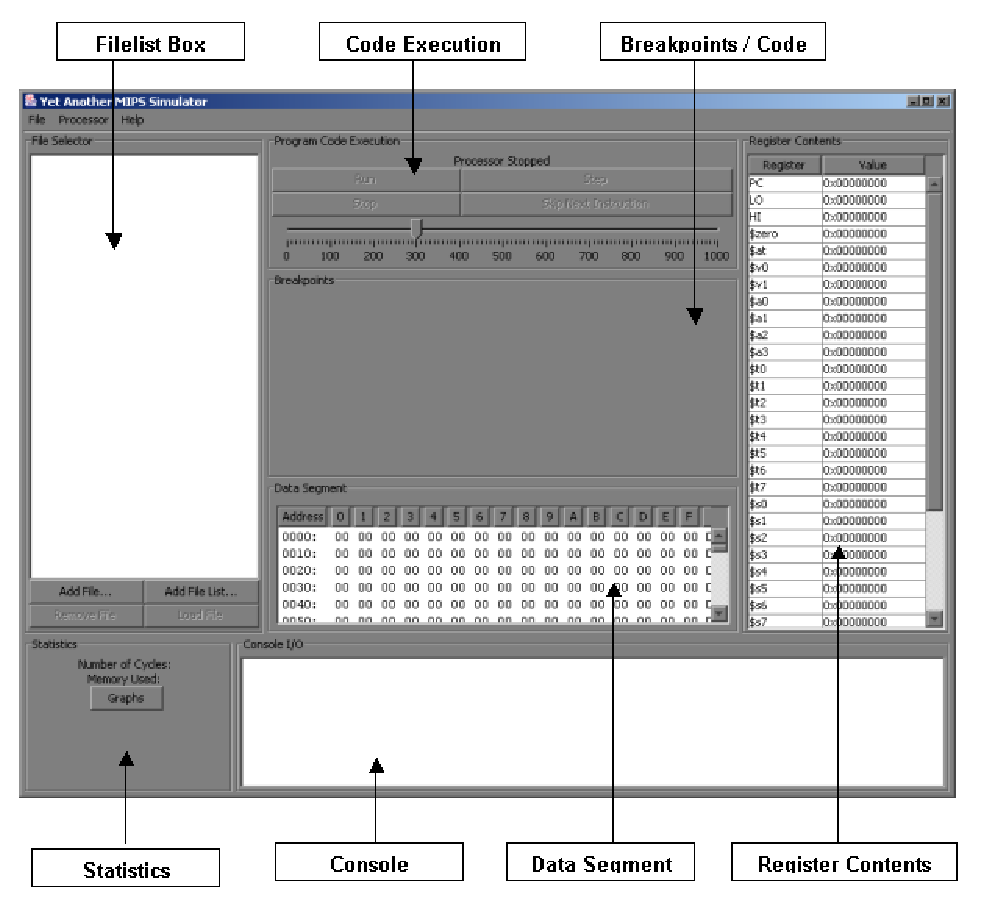
\includegraphics[scale=0.5]{Ch4-Fig2.eps}
\caption{Graphical User Interface}
\label{figure.GUI}
\end{figure}



\subsection{Adding Files to the File Selector Box}
If input files were specified at the command line, they will be displayed in the File Selector Box. Otherwise, files can be added to the File Selector Box by clicking Add File and then using the dialogue box to add a file.

\begin{figure}[h]
\centering
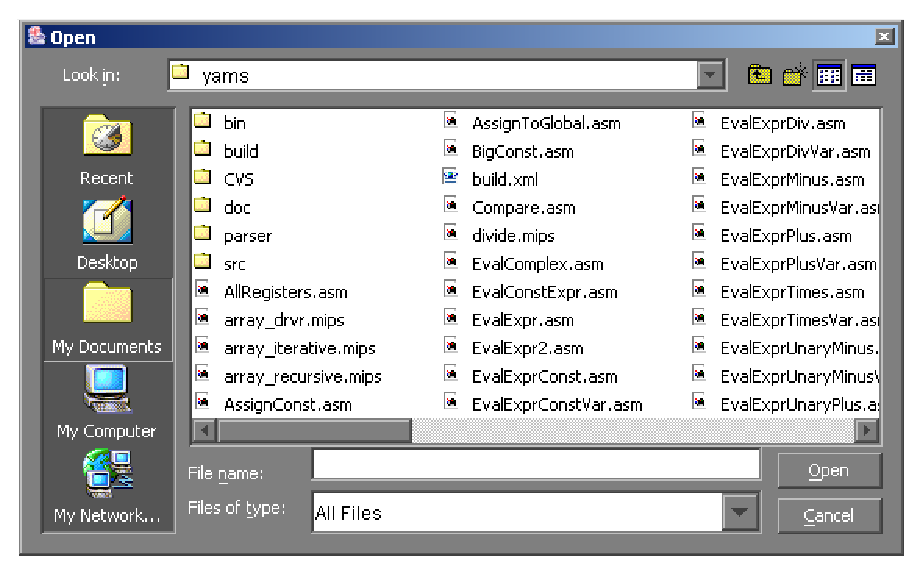
\includegraphics[scale=0.5]{Ch4-Fig3.eps}
\caption{Adding a File}
\label{figure.Adding a File}
\end{figure}

Here you can select an assembly file to load into the simulator.

To add a list of files, click the 'Add Filelist' button, and select the file that contains the list of assembly files you wish to load.  The filelist should contain the file names of the assembly files, one per line.

If you wish to remove a file from the list, select it in the list box, then click the Remove File button below.


\subsection{Loading a File}
Once you have chosen the file you wish YAMS to simulate, you can then load the file by pressing the 'Load File' button.

The program code, memory locations and register contents are shown once the file is loaded, as can be seen below, with the first line of code highlighted.

\begin{figure}[h]
\centering
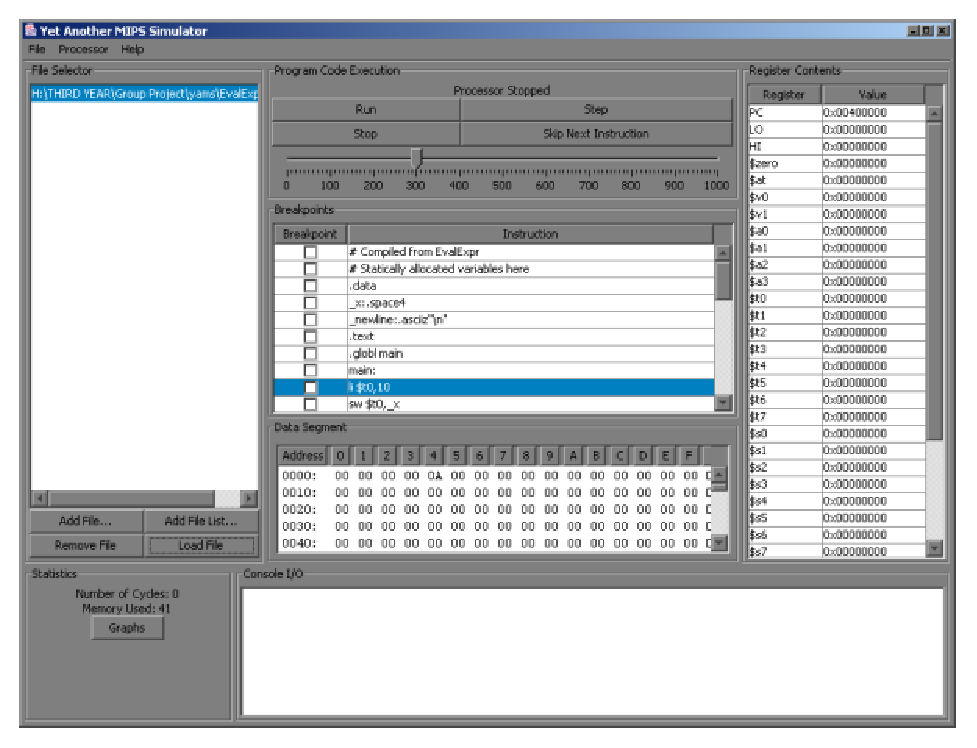
\includegraphics[scale=0.5]{Ch4-Fig4.eps}
\caption{Loading a File}
\label{figure.Loading a File}
\end{figure}


\subsection{Adding Breakpoints}
Adding a breakpoint to the program is simple.  Just use the checkbox that is next to the line you where you wish to pause execution.  When the simulator reaches here, you can examine  the contents of the register and memory locations.

\subsection{Controlling Execution}

\begin{figure}[h]
\centering
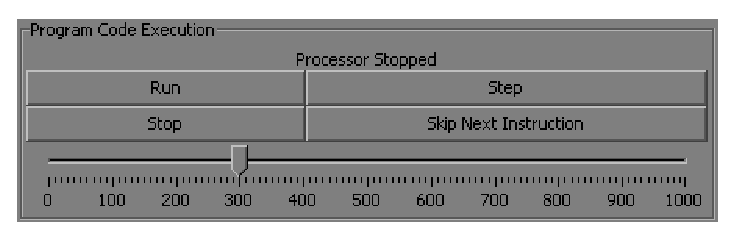
\includegraphics[scale=0.5]{Ch4-Fig5.eps}
\caption{Controlling Execution}
\label{figure.Controlling Execution}
\end{figure}

\subsubsection{Speed}
The speed of the processor can be controlled by the slider bar - a larger value means a longer gap between each instruction so you are able to execute the program in 'slow motion'.  

\subsubsection{Run}
Press the Run button to begin the execution of the assembly program.  The execution of the program is done slowly line by line so that you can see each line being executed individually and the contents of the registers and memory changing.  The current line being executed is shown by the highlighted line in the program code.

\subsubsection{Stop}
To Stop the execution of the program, press the 'Stop' button.  The instruction that is currently being executed will remain highlighted.  From here, it is possible to resume the execution of the program by pressing 'Run', run just the next instruction by pressing 'Step' or skip the next instruction by pressing the 'Skip Next Instruction' button.

\subsubsection{Single Step}
If you wish to single step each line of the program, first of all, press the Stop button which will pause the programs execution.  It is then possible to use the Step button to execute each instruction one at a time.  Note that one line of assembly code can be made up of several processor operations, so pressing Step will not always move to the next instruction, but will execute the next processor operation for that line.

\subsubsection{Skip}
Pressing 'Skip Next Instruction' will ignore the next insturction that is to be executed.  It is recommended that this feature is used while in stepping mode so that it can be seen clearly which instruction is to be skipped.


\subsection{Interpreting Output}


\subsubsection{Console Output}
The Console I/O box is used for 2 things:
- Error messages from the parser - if an error was encountered while parsing the assmebly file, the type of error and related line number are displayed.  Correct the error then try loading the file again.

- Output of the program - during the execution of the program, any output is displayed in the Console I/O box.

\subsubsection{Statistics}
Statistics for the run of the program are available in the Statistics Panel of the interface.  This shows the number of CPU cycles required so far for the program executing, and the total amount of memory used by the program.  These are updated constantly as the program is executed.

\begin{figure}[h]
\centering

\includegraphics[scale=0.5]{Ch4-Fig6.eps}
\caption{Statistics Panel}
\label{figure.Statistics Panel}
\end{figure}


Pressing the 'Graph' button will display a window with 2 tabs:
- How many times each register was used
- How many times each line was executed

This can be useful in seeing where loops are in the program as the lines in the loop are executed more often than the rest of the instructions.



\section{Adding Instructions}


The core functionality of YAMS is extensible and has been designed so that advanced users can add new instructions to its framework. The purpose of this aspect to the application is to provide flexibility, users can add new Regular and Pseudo instructions to the system. This is to cater for the differing standards within MIPS instruction sets and allows the application to be specifically adapted to certain situations (i.e. restrict the instructions that can be used to encourage low-level optimisation of programs). A potential further extension of this implies that an entirely new instruction set (different to MIPS) could be developed and tested within the YAMS framework, taking into account the restraints of the MIPS processor.

The following guide will explain how to add a new instruction to the existing application, providing information on the three specific areas such an addition will have a significant impact upon: the Parser, the Assembler and the Processor.




\subsection{Overview}

Fundamentally the process of adding an instruction can be broken down into four main stages:

\begin{enumerate}
\item Parser Extension
\item Assembler Extension
\item Processor Extension
\item Building
\end{enumerate}




\subsection{YAMS and XML}

As has already been mentioned, YAMS has been designed to work flexibly with different instruction sets. To achieve this, a central XML repository of data regarding each instruction is maintained within the application containing all relevant details and some code. The various software components behave according to the data contained within this repository. This behaviour is achieved in two main ways:


\begin{enumerate}

\item Specific Java Code

Some project components will require specific code handlers to determine their behaviour on encountering a specific instruction. YAMS has been designed such that this code can be directly contained within \verb"<Javacode></Javacode>" within the XML file. XSLT will then be used to re-generate the specific classes required for YAMS to handle the newly added instructions. Thus, it will be necessary to perform a recompilation of YAMS before the changes to the project will take effect.

Software components affected: Parser, Processor (Instruction and System-call Handlers)

\item Real-time XML Parsing

Some project elements will not require specific code, and instead need only to refer to the data contained within the XML Repository. In these situations, we can make use of XML DOM parsing to read in the data from the file at startup and fill object tables with the required information.

Software components affected:	Assembler, Statistics Manager (Processor sub component)

\end{enumerate}


Therefore, to add a new instruction (or manipulate the current instruction set), the advanced user need only design the instruction, modfiy the XML file and then recompile YAMS. There are specific scripts available within the YAMS package to make this as user-friendly as possible.

\subsection{Step-by-step Design / Addition of Instruction}

The following guide  explains how to add an instruction to the system step-by-step (R steps are REQUIRED fields that are needed by YAMS). When constructing the XML representation it would be useful to refer to the quick-reference tables included at the conclusion of this section of the guide, which will indicate which tags need to be filled out for which instruction, and their allowed content types.

The general XML structure required is shown in figure \ref{figXMLTemplate}.

\begin{figure}[]
\begin{center}
\begin{verbatim}
<Instruction>
  <Name> ......... </Name>
  <OperandTypes> ......... </OperandTypes>
  <Type fixedRt="BOOLEAN"> ......... </Type>
  <Javacode></Javacode>
  <CoreMachineCode> ......... </CoreMachineCode>
  <MachineCodeRepresentations>
    <Representation>
      <OperandsCoding> ......... </OperandsCoding>
      <MachineCode> ......... </MachineCode>
      <Operands>
        <Op>
          <Number> ......... </Number>
          <Type> ......... </Type>
          <Mask> ......... </Mask>
          <EncodeBits> ......... </EncodeBits>
          <OutputBits> ......... </OutputBits>
          <OffSetMode> ......... </OffSetMode>
        </Op>
        ......
      </Operands>
    </Representation>
    ......
  </MachineCodeRepresentations>
  <Help>
    <FullName></FullName>
    <Format></Format>
    <Description></Description>
  </Help>
</Instruction>
\end{verbatim}
\end{center}
\caption{XML Template}
\label{figXMLTemplate}
\end{figure}


\subsubsection{FRAMEWORK MODIFICATION}

Some parts of the XML Instruction representation are generic, and will be used by multiple software components within YAMS (Parser,Assembler,Processor), these tags are described below.

\begin{enumerate}
\setcounter{enumi}{0}


\item R - Instruction Name: \verb"<Name>"

This field contains the name of the instruction, as will be used within the MIPS code e.g. "add","neg" etc.


\item R - Type: \verb"<Type>"

Tells Assembler/Processor/Parser what type of instruction this in terms of structure. This is the FIRST major instruction decision to be made, and will have an impact on other sections of the XML.



\begin{description}

\item[Regular]

A REGULAR INSTRUCTION has one set of possible operands, therefore one machine code representation.

Details on regular instructions are required in the following software components:
\begin{itemize}
\item included in parser (usable in mips code)
\item included in assembler (encoded to machine code)
\item included in processor (processor knows what specific steps to take to execute this instruction)
\end{itemize}

\item[Extended]

An EXTENDED INSTRUCTION has multiple representations depending on the different operand combinations, thus will require and entry for the Core Machine Code field.

More than one set of possible operands e.g. add REG REG REG / add REG REG IMMEDIATE -> One machine code representation per possible operand construct NOT a pseudoinstruction because underlying instruction is still atomic but for some operand representations, other steps have to be taken to cater for the different operand before the core function is executed

e.g. there is a specific instruction machine code representation add REG REG REG = 00-9o-0os, however if add REG REG IMMEDIATE is required as a variation on this instruction a li REG IMMEDIATE must 'first' be executed before the regular add can be made. To cater for this	conceptual difference, these are called Extended instructions.

NB with extended instructions, since they still have a core instruction (e.g. add still has atomic underlying expression) it is now NECESSARY to fill in the CoreMachineCode tag (described in a moment) included in parser (usable in mips code).

Details on extended instructions are required in the following software components:
\begin{itemize}
\item included in parser (instruction is usable in mips code)
\item included in assembler (encoded to machine code)
\item included in processor (processor knows what specific steps to take to execute the CORE VERSION of this instruction)
\end{itemize}

\item[Pseudoinstruction]

A PSEUDOINSTRUCTION is not specifically executed by processor,rather is made up of other atomic instructions.

Can be one set of operands or more than one set of operands (and therefore representations), and has no core representation (i.e. there is no explicit core machine code representation for this instruction). Therefore it is composed of a series of other atomic instructions that overall have the required effect of the instruction. It will not be known the processor, since it will already know the core instructions it uses.

Details on pseudoinstructions are required in the following software components:
\begin{itemize}
\item included in parser (usable in mips code)
\item included in assembler (encoded to machine code)
\item NOT included in processor
\end{itemize}

There also exists an attribute for the Type tag which must be filled in as fixedRt="true" for instructions

The fixedRt attribute must be set to true for I type branch instructions that use the Rt field of the instruction to identify the branch type. This attribute is require to identify these instructions for requiring extra decoding in the Instruction Handler. 
The only MIPS instructions to require this attribute are: bltz, bltzal, bgez and bgezal.

If the attribute is not specified, the default value is false.



\end{description}


\item D - Core Machine Code : \verb"<CoreMachineCode>"

This is ONLY required when an Extended instruction is created (multiple representations depending on operands, while using underlying machine code representation). It contains the machine code for the actual instruction, not including an pre-instruction execution steps that need to occur for more complicated combinations of operands e.g. add REG REG REG has a specific machine code representation, but add REG REG IMMEDIATE uses this representation plus some other atomic instructions to cater for the different operands.

The value of this field should be the simplest representation within the MachineCodeRepresentations/Representation/MachineCode tag, and should be 1 x 32 bit machine word.


\end{enumerate}


\subsubsection{PARSER MODIFICATIONS}

The Parser will use method 1 (see earlier) to obtain the information from the XML file. Essentially it will use an XSLT transformation to convert selected data fields contained within the XML to parts of the Parser handler. This handler will deal with recognising an instruction and will be able to instruct the parser how to recognise and validate the presented instruction. This information includes the name of the instruction, and the possible operands that it takes. The following field is solely used by the Parser in this respect:

\begin{enumerate}
\setcounter{enumi}{3}

\item R - Operand Types : \verb"<OperandTypes>"


This indicates to the parser what number and type of operands are being used for the specified instruction. For the purposes of parsing (decided to be more of a syntax check than a semantic check, which will be dealt with more within the assembling phase), there are four main operand types:

\begin{description}

\item[Operand.TYPE\_REGISTER]
Indicates the operand is a register (from available list in MIPS architecture)
\item[Operand.TYPE\_IMMEDIATE]
Operand is an immediate (NB encompasses all forms of immediates, no range checking this occurs within the assembler)
\item[Operand.TYPE\_LABEL]
Operand is a Label (String referring to another point within the program)
\item[Operand.TYPE\_ADDRESSING]
Operand is an Addressing Operand, referring to some address within memory. This can take one of 6 sub-forms (please consult MIPS addressing documentation and following table for further information):

\end{description}

The addressing mode can either be an absolute value, an offset from the current text address or an offset from a fixed block address (for YAMS it is 0x10008000 in main memory).

Key: where I(R) = I+R

\begin{table}[]
\begin{center}
	\begin{tabular}{|l|p{3in}|}
		\hline
		Type & Addressing Mode \\
		\hline
		Immediate & 16 bit Immediate offset, 32 bit Absolute address \\
		Immediate(Register) & Immediate (16/32 bit) plus register value gives absolute address \\
		Register & Register value gives absolute address \\
		Label & Label (Evaluate offset) \\
		Label+-Immediate & Label (Evaluate offset) +- 16/32 bit offset \\
		Label+-Immediate(Register) & Label (Evaluate offset) +- 16/32 bit offset \\
		\hline
	\end{tabular}
\caption{Addressing Modes}
\end{center}
\end{table}



This will tell the parser exactly what operands to expect when an instruction of this type is presented within the MIPS code. To specify a representation, place comma separated operand types (in corresponding order to desired instruction) within the <OperandTypes></OperandTypes> tags.

Cardinality:

\begin{itemize}
\item For Regular instructions there will only be one valid operands representation, thus one \verb"<OperandTypes>" entry.
\item For Extended/Pseudoinstructions there can be more than representation for the operand types thus there will be a corresponding \verb"<OperandTypes>" entry for each one.
\end{itemize}

Example: Instruction Name = add

\begin{verbatim}
Regular Add instruction dealing with registers
<OperandTypes>Register,Register,Register</OperandTypes>
Add instruction allowing an immediate to be included
<OperandTypes>Register,Register,Immediate</OperandTypes>
\end{verbatim}

\end{enumerate}



\subsubsection{ASSEMBLER MODIFICATIONS}


The assembler requires complex and specific information regarding the structure and operand types involved in an instruction. It utilies method 2 to obtain information from the XML file, reading it on startup, parsing the information and loading it into table objects for further reference to during the assembling phase. The following sections must be specifically included to tell the assembler exactly what to do with the operands you provide it.


\begin{enumerate}
\setcounter{enumi}{4}

\item R - Machine Code Representations: \verb"<MachineCodeRepresentations>"

The assembler needs to know what the specific machine code representation(s) for the current instruction is (are).

If the instruction is a Regular Instruction, then there must be ONLY ONE Representation node within this higher level tag. If however, the instruction is an Extended or Pseudo Instruction, then there must be more of these representations to cope with the different alternatives.


Operand Semantic Differences

It is important to note, that when we come to defining the details of the instruction for the assembler, our notion of operands must change slightly. Within the parser operand definition tags (\begin{verbatim}<OperandTypes>\end{verbatim}) we only consider there to be four possible operand types. However, the assembler must take into account the fact that there will in fact be different machine code representations for separate instructions using the same parser operand type.

For example, the parser has no notion of there being a difference between a 16 and 32 bit integer, however when it comes to assembling we can only deal with 16 bit integers in the majority of our operations. Thus we must solve this problem by using other commands to load in order the bottom half and top half of 32 bit integers into a register. Once there we can manipulate it to perform the required operation. So that our generated code remains optimal (i.e instructions using only 16 bit immediates dont need to perform as many instructions as 32 bit immediates will), we separate dealing with 16 and 32 bit immediates into different \begin{verbatim}<Representation>\end{verbatim} tags.

The required contents of the \begin{verbatim}<Representation>\end{verbatim} node(s) within this lower level will be discussed within this section, but essentially they are differentiated from each other by an encoded representation of the operands (discussed later) and any further details regarding these operands are contained within its \begin{verbatim}<Operands>\end{verbatim} tag. The following example illustrates this and the points discussed regarding the operands.

e.g. "add" instruction has two <OperandType> tags and thus must have two representation tags to correspond to these:

\begin{verbatim}
....

<OperandType>Register,Register,Register</OperandType>
<OperandType>Register,Register,Immediate</OperandType>

....

<MachineCodeRepresentations>
  <Representation>
    <OperandsCoding>111</OperandsCoding>
    <MachineCode>000000bbbbbcccccaaaaa00000100000</MachineCode>
    <Operands>
    </Operands>
  </Representation>
  <Representation>
    <OperandsCoding>110</OperandsCoding>
    <MachineCode>001000bbbbbaaaaacccccccccccccccc</MachineCode>
    <Operands>
      <Op>
        <Number>3</Number>
        <Type>0</Type>
        <Mask>1111111111111111</Mask>
        <EncodeBits>16</EncodeBits>
        <OutputBits>16</OutputBits>
        <OffSetMode>2</OffSetMode>
      </Op>
    </Operands>
  </Representation>
  <Representation>
    <OperandsCoding>11a</OperandsCoding>
    <MachineCode> 00111100000aaaaadddddddddddddddd
                  001101aaaaaaaaaacccccccccccccccc
                  000000bbbbbaaaaaaaaaa00000100000
    </MachineCode>
    <Operands>
      <Op>
        <Number>3</Number>
        <Type>a</Type>
        <Mask>11111111111111111111111111111111</Mask>
        <EncodeBits>32</EncodeBits>
        <OutputBits>32</OutputBits>
        <OffSetMode>2</OffSetMode>
      </Op>
    </Operands>
  </Representation>
</MachineCodeRepresentations>
\end{verbatim}

As can be seen from the above example, "add" only has two possible parser configurations:

add REGISTER REGISTER REGISTER \\
add REGISTER REGISTER IMMEDIATE

However, the immediate in the second instruction could be dealt with differently depending on whether it is a 16 bit or a 32 bit immediate, as has been reflected by the fact that there are THREE <Representation> nodes and only TWO <OperandType> nodes. Therefore as can be seen there are conceptually different concepts between how the Parser and Assembler see operands, and when designing an instruction it would be a good idea to deal with the sections differently.

Please note it is also perfectly possible to restrict the use of immediates to only 16 bit integers, by only including its representation and not the code for 32 bit integer representations. Given this information in the XML, YAMS will infer that the instruction is designed to only take 16 bit ntegers and will throw an error when presented with 32 bit ones instead.

Representation

The basic structure of a <Representation> node is highlighted below:

\begin{verbatim}
<Representation>
  <OperandsCoding> ......... </OperandsCoding>
  <MachineCode>
  .................
  </MachineCode>
  <Operands>
    <Op>
      <Number> ..... </Number>
      <Type> ..... </Type>
      <Mask> ................... </Mask>
      <EncodeBits> ..... </EncodeBits>
      <OutputBits> ..... </OutputBits>
      <OffSetMode> ..... </OffSetMode>
    </Op>
  </Operands>
</Representation>
\end{verbatim}

When adding an instruction, as has already been mentioned, you must add Representation nodes for each of the different operand combinations that there will be (from extended Operand set).

For each representation we must fill out the following information:

\begin{enumerate}

\item Operands Coding

Each representation is uniquely identified by a string of characters which represent the operand types that this representation of the instruction will be catering for. The following table contains the available operand types that we can use in our operand code:

Table : Operand Coding Set

Contains a list of available operand codes that we can use to uniquely describe our representation. As has already been mentioned there are differences between the Parser and Assembler representations of operands, and the following table matches the two distinct sets.


\begin{table}[]
\begin{center}
	\begin{tabular}{|p{0.5in}|l|p{1.5in}|}
	\hline
	Character Code & Meaning & Corresponding Parser Operand \\
	\hline
	0	&	<=16 Bit Twos Complement Immediate		&	Immediate \\
	a	&	32 Bit Twos Complement Immediate		&	Immediate \\
	1	&	Register								&	Register \\
	2	&	Label									&	Label \\
	3	&	Address									&	Addressing \\
	4	&	Add: Immediate							&	Addressing \\
	5	&	Add: Immediate(Register)				&	Addressing \\
	6	&	Add: Label								&	Addressing \\
	7	&	Add: Label\_Plus\_Immediate				&	Addressing \\
	8	&	Add: Label\_Plus\_Immediate\_Register	&	Addressing \\
	c	&	Add: Label\_Minus\_Immediate\_Register	&	Addressing \\
	9	&	Add: Register							&	Addressing \\
	b	&	no operands								&	Addressing \\
	\hline
	\end{tabular}
\caption{Operand Coding Set}
\end{center}
\end{table}

Example: for the "add" instruction

\begin{enumerate}
\item add REGISTER REGISTER REGISTER has only one possible representation for registers, thus \verb"<OperandCode>111</OperandCode>"
\item add REGISTER REGISTER IMMEDIATE has two possible representations, 16/32 bit immediates, thus
\begin{verbatim}
	a)	<OperandCode>110</OperandCode>
	b)	<OperandCode>11a</OperandCode>
\end{verbatim}

\end{enumerate}
	
\item MachineCode

The representation will contain a <MachineCode> tag which contains the underlying machine code required to carry out the instruction. However, before receiving the actual instruction it is impossible to identify what the values of these operands are. Therefore the machine code will contain "gaps" in specific parts, which can be filled in by the assembler when it works out the actual values of each operand. These actual values need to be mapped into their correct "gaps" in the code. Thus within the XML file, these gaps are represented as string of characters (from following table) of the required length.


\begin{table}[]
\begin{center}
	\begin{tabular}{|l|l|}
	\hline
	Character	&	Operand Number \\
	\hline
	a	&	1 \\
	b	&	2 \\
	c	&	3 \\
	d	&	4 \\
	e	&	5 \\
	f	&	6 \\
	g	&	7 \\
	h	&	8 \\
	i	&	9 \\
	j	&	10 \\
	\hline
	\end{tabular}
\caption{Characters used within strings to indicate a position for operand substitution by the assembler}
\end{center}
\end{table}


As can be seen, YAMS has been designed to cater for instructions with up to 10 operands if necessary.

Example : In YAMS, given an instruction

instruction OPERAND\_1 OPERAND\_2 OPERAND\_3

the assembler will retrieve the required representation from the Pre-Loaded XML Tables by working out the required operand code (see above) for this specific "instruction." This will return a pre-defined machine code representation with "gaps" where the computed operands need to go. The assembler thus calculates the machine code values of the user supplied operands and then one-by-one substitutes their values into the required places in the machine code. For example, the machine code for our generic "instruction" example is as follows

010010aaaaabbbbbccccc00000111111

YAMS will then calculate the values of OPERAND\_1,\_2 and \_3 and then map them to their correct positions within the code.

OPERAND\_1 = 00001 = aaaaa
OPERAND\_2 = 00100 = bbbbb
OPERAND\_3 = 11111 = ccccc

01001000001001001111100000111111

Therefore during the design of an instruction, effort must be made to ensure that the correct operand gaps are left in the right places ready for substitution at run time.


\item Operands

As has been seen, the specific type of the operand (e.g. immediate, label etc) has already been decided upon for the current instruction being added. However, the assembler will require further information on some of these operands in order to calculate their values correctly.

For example if we have an Immediate value for one of the operands, it is possible we may not want to include all of this immediate value when we write it to memory. Such a situation may occur when considering offsets. If our immediate is a value of 400 bytes = 110010000 bytes, since we are using aligned memory access, then we could feasibly drop the last 2 bytes of our immediate and save some space for further information in our instruction. In such cases, YAMS provides the facility for an instruction
writer to tell the assembler to do so.

However, this only applies to some of the operand types that we are using, the following table indicates for which Operands an \verb"<Op>" tag should be included.

\begin{table}[]
	\begin{tabular}{|l|l|p{1in}|}
	\hline
	Operand	&	Description	&	Required \verb"<Op>" Description? \\
	\hline
	0	&	$<=$16 Bit Twos Complement Immediate		&	Yes \\
	a	&	32 Bit Twos Complement Immediate			&	Yes \\
	1	&	Register									&	No \\
	2	&	Label										&	Yes \\
	3	&	Address										&	Yes \\
	4	&	Add: Immediate								&	Yes \\
	5	&	Add: Immediate(Register)					&	Yes \\
	6	&	Add: Label									&	Yes \\
	7	&	Add: Label\_Plus\_Immediate					&	Yes \\
	8	&	Add: Label\_Plus\_Immediate\_Register		&	Yes \\
	c	&	Add: Label\_Minus\_Immediate\_Register		&	Yes \\
	9	&	Add: Register								&	Yes \\
	b	&	no operands									&	No \\
	\hline
	\end{tabular}
\caption{Requirement for Op Tags for Operand Types}
\end{table}

For each of the YES cases above, an \verb"<Op>" tag must be filled out as set out below:

Operands

An Operand tag takes the following form:

\begin{verbatim}
<Op>
	<Number> ..... </Number>
	<Type> ..... </Type>
	<Mask> ................... </Mask>
	<EncodeBits> ..... </EncodeBits>
	<OutputBits> ..... </OutputBits>
	<OffSetMode> ..... </OffSetMode>
</Op>
\end{verbatim}

Essentially, the assembler has already been told what machine code representation it has to map the operands to, and the information contained within the \verb"<Op>" tags for each operand explains to what level of accuracy to perform calculations, what offset mode to be using if we are calculating symbolic labels and which specific bits to use in the final substitution.

\begin{enumerate}

\item Number

This refers to which operand within the \verb"<OperandCode>" we are referring to, via indexing. The first operand takes a Number=1, the second Number=2 and so on.

\item Type

This refers to the operand type which we are placing constraints upon (from extended Assembler Operand Type list described already)


Example: for the "add" instruction, under the 11a representation, the XML will contain:

\begin{verbatim}
<Op>
	<Number>3</Number>
	<Type>a</Type>

	.....
\end{verbatim}

\item Encode Bits

This field specifies to how many bits we wish to encode the binary value which YAMS' Operand Handler will be calculating the current operand to.
YAMS will thus throw an error if the provided value cannot be represented within this range. For example, for a Label operand, we are dealing with an 16 bit "gap" in which we can place our offset. Therefore if we encode to 16 bits accuracy we make sure that the label is within our addressable range.

The number of Encode Bits must be >= OutputBits field (number of bits we use in the substitution).

\item Mask

The Mask will highlight which bits of the encoded representation we wish to include in the final output for our operand (the value we will actually be substituing into the predefined machine word. This is done bitwise:

1 (at index i)	Indicates that the encoded bit at index i IS included in the substituting value
0 (at index i)	Indicates that the encoded bit at index i IS NOT included in the substituting value

Therefore, the restriction here is that the number of 1s in the Mask must be equal to the OutputBits field.

For example, to mask out the bottom two bits of a 16 bit number, use 1111111111111100 as the Mask value.

\item Output Bits

This indicates the final number of bits that we will be using as the substituting bit string (the final value we substitute into the machine word as the operand). It must equal the number of 1s we have in the Mask field.

\item Off Set Mode

For certain operands (e.g. Labels), the value of the provided operand that we want to place into our instruction will need to be a calcualated offset. This offset can be from the current line address or maybe from the fixed block address of 0x10008000 used in MIPS. On other occasions we may want to calculate the absolute address. Therefore, YAMS provides instructions with three calculation modes for their operands, as below:

\end{enumerate}

\begin{table}[]
\begin{center}
	\begin{tabular}{|l|l|p{2.5in}|}
	\hline
	Mode	&	Title	&	Description \\
	\hline
	0	&	Current Position Mode		&	Will calculate the offset based on the current line address (e.g. jump) \\
	1	&	Block Address Mode			&	Calculates offset from 0x10008000 \\
	2	&	Absolute Address Mode		&	Calculates the absolute address of the operand \\
	\hline
	\end{tabular}
\caption{Offset Modes For Operands}
\end{center}
\end{table}

\end{enumerate}
\end{enumerate}

\subsubsection{PROCESSOR MODIFICATIONS}

The processor must be able to handle instructions correctly, and the XML file will contain all the data regarding each instruction. The processor will read this data using Method 1, so at compile time the java code contained within the XML should be able to be placed within the Processor Instruction Handlers. This code is contained within the \verb"<Javacode>" tag for each instruction, highlighted below.

\begin{enumerate}
\setcounter{enumi}{5}

\item D - Javacode: \verb"<Javacode>"

For newly added REGULAR and EXTENDED instructions, the processor will have to be able to carry out some new functionality in order to execute the required behaviour for the specific instruction. However, for PSEDUOINSTRUCTIONS, this will not be necessary since they will be defined in terms of already existing instructions.



\begin{table}[]
\begin{center}
	\begin{tabular}{|l|l|}
	\hline
	Instruction Type	&	Javacode Tag \\
	\hline
	Regular				&	Required \\
	Extended			&	Required \\
	Pseudoinstruction	&	Not Required \\
	\hline
	\end{tabular}
\caption{Requirements For Javacode Modification}
\end{center}
\end{table}

In order to implement the functionality of a new instruction, it will be necessary to understand the functions available to this new instruction through the processor. There are interfaces available in the YAMS procesor documentation that highlight the features of the simulated mips processor, and they can be used to construct the java code appropriately.

For an instruction to be handled by the processor correctly it should have a valid and unique machine code representation. For Regular instructions, this is described in the MachineCode tag in the MachineCodeRepresentation. For Extended instructions, this is found in the CoreMachineCode tag.
The processor does not generate handling code for pseudoinstructions, for these are assembled into their consitituent instructions before they can be executed.

Java code is used to describe the semantics of the instruction. The semantics will likely include reading values to/from registers and/or memory, depending on what the instruction is designed to do. The code is placed inside the <Javacode> opening and </Javacode> closing tags.

Before writing any Java code, it is recommended to be familiar with the section of this report that describes the InstructionHandler component of the Processor. Depending on the type of MIPS instruction (R, I or J) that is being added, the interfaces and variables available to the programmer vary. 

Tables \ref{tab:PInterfaces}, \ref{tab:RType}, \ref{tab:IType} and \ref{tab:JType} show the processor interfaces and variables available, by type of 


\begin{table}
\begin{center}
	\begin{tabular}{|l|l|l|}
	\hline
	mem		&	MemoryManagerInterface		&	the memory manager \\
	regs	&	RegisterManagerInterface	&	the register manager \\
	stats	&	StatisticsManagerInterface	&	the statistics manager \\
	out		&	PrintStream					&	the console output \\
	verbose	&	PrintStream					&	the verbose output \\
	op		&	int							&	the 'op' bitfield \\
	op\_bitstr&	MIPSBitstring				&	ditto (as bitstring) \\
	\hline
	\end{tabular}
\caption{Processor Interfaces}
\label{tab:PInterfaces}
\end{center}
\end{table}


\begin{table}
\begin{center}
	\begin{tabular}{|l|l|l|}
	\hline
	rs			&	int				&	the first source register \\
	rs\_bitstr	&	MIPSBitstring	&	ditto (as bitstring) \\
	rt			&	int				&	the second source register \\
	rt\_bitstr	&	MIPSBitstring	&	ditto (as bitstring) \\
	rd			&	int				&	the destination register \\
	rd\_bitstr	&	MIPSBitstring	&	ditto (as bitstring) \\
	shamt		&	int				&	the shift amount \\
	shamt\_bitstr&	MIPSBitstring	&	ditto (as bitstring) \\
	func		&	int				&	the 'func' bitfield \\
	func\_bitstr	&	MIPSBitstring	&	ditto (as bitstring) \\
	\hline
	\end{tabular}
\caption{R type only}
\label{tab:RType}
\end{center}
\end{table}



\begin{table}
\begin{center}
	\begin{tabular}{|l|l|l|}
	\hline
	rs			&	int				&	the first register \\
	rs\_bitstr	&	MIPSBitstring	&	ditto (as bitstring) \\
	rt			&	int				&	the second register \\
	rt\_bitstr	&	MIPSBitstring	&	ditto (as bitstring) \\
	i			&	int				&	the SIGN-EXTENDED version of 'immediate' bitfield \\
	i\_bitstr	&	MIPSBitstring	&	the 'immediate' bitfield as bitstring \\
	\hline
	\end{tabular}
\caption{I type only}
\label{tab:IType}
\end{center}
\end{table}



\begin{table}
\begin{center}
	\begin{tabular}{|l|l|l|}
	\hline
	addr		&	int				&	the 'addr' bitfield \\
	addr\_bitstr	&	MIPSBitstring	&	ditto (as bitstring) \\
	\hline
	\end{tabular}
\caption{J type only}
\label{tab:JType}
\end{center}
\end{table}



The Java code should be placed between the \verb"<Javacode>" and the \verb"</Javacode>" tags.

What the Java code for new instructions should NOT contain:
\begin{itemize}
\item return statements
\item frivolous use of the 'out' PrintStream
\item attempts to reference classes outside the yams.processor package
\item attempts to use interfaces/variables not accessible for the instruction type (R, I or J)
\end{itemize}

Violations of these recommendations will cause either a failure at XSLT transformation stage or when compiling the generated InstructionHandler.java file.

{\bf N.B. All special characters, such as \verb"&" (ampersand), \verb"<" (left chevron) and \verb">" (right chevron) MUST be converted to their HTML equivalent.}
\begin{verbatim}
&  ->  &amp;
<  ->  &lt;
>  ->  &gt;
\end{verbatim}
This is because XSLT has its own individual use for these characters in XSLT files.

Failure to do this conversion for all special characters will result in the following error on applying the transformation during the build process.

\begin{quote}
{\tt
[xslt] : Fatal Error! org.xml.sax.SAXParseException: Illegal character or entity reference syntax. Cause: org.xml.sax.SAXParseException: Illegal character or entity reference syntax.
}
\end{quote}

Example Javacode for existing instructions:
\begin{verbatim}
  'add rd, rs, rt' (addition)
  'div rs, rt' (divide)
  'beq rs, rt, label' (branch on equals)

<Instruction>
  <Name>add</Name>
  ...
  <Javacode>
    regs.setReg(rd, regs.getReg(rs) + regs.getReg(rt));
  </Javacode>
  ...
</Instruction>

<Instruction>
  <Name>div</Name>
  ...
  <Javacode>
    int quotient;
    int remainder;
    int rscontents = regs.getReg(rs);
    int rtcontents = regs.getReg(rt);
    quotient = rscontents / rtcontents;
    remainder = rscontents % rtcontents;
    regs.setReg("LO", quotient);
    regs.setReg("HI", remainder);
  </Javacode>
  ...
</Instruction>

<Instruction>
  <Name>beq</Name>
  ...
  <Javacode>
    if(regs.getReg(rs) == regs.getReg(rt)) {
      int pc = 0;
      pc = regs.getReg("PC");
      pc += i * 4 - 4;
      regs.setReg("PC", pc);						
    }
  </Javacode>
  ...
</Instruction>
\end{verbatim}

\item R - Help Modification: \verb"<Help>"

The final stage to adding an instruction would be to add the help tags, so that the help documentation can be created appropriately:

\begin{verbatim}
<Help>
  <FullName></FullName>
  <Format></Format>
  <Description></Description>
</Help>
\end{verbatim}


\end{enumerate}



\subsection{Building The Project}

As mentioned in the YAMS spec. YAMS is built in such a way the
adding and removing instructions can be done without modifying any
YAMS' program code.

You'll, obviously, need to get the source code bundle.

\subsubsection{Software Requirement}

Apache Ant is required for building YAMS.

To check whether Ant is installed on the system, type in
console:

\texttt{\$ ant -version}

If you see something similar to:

\texttt{Apache Ant version 1.5.3 compiled on April 16 2003}

You are good to go on and start the build, otherwise, please
install Ant from the {\tt /extras} directory in the YAMS distribution.  An installation guide can be found at {\it http://ant.apache.org}

\subsubsection{Doing the build}

Running the following command in the root directory or the YAMS
distribution (that is, where the \texttt{build.xml} locates) will
build a YAMS.jar file in the build directory:

\texttt{\$ ant}

Simple as that, your new customized YAMS is there waiting to be
run.










\subsubsection{QUICK-REFERENCE PAGE for adding an instruction}


The following quick-reference tables give an overview of how to add an insruction to the YAMS application:

\noindent \textbf{PARSER TABLE}

Table \ref{tab:Parser} shows the operand types used by the Parser.

\begin{table}[]
\begin{center}
	\begin{tabular}{|l|}
	\hline
	Type \\
	\hline
	Operand.TYPE\_REGISTER \\
	Operand.TYPE\_IMMEDIATE \\
	Operand.TYPE\_LABEL \\
	Operand.TYPE\_ADDRESSING \\
	\hline
	\end{tabular}
\caption{$<$OperandType$>$ Tag Comma Separated Available Types}
\label{tab:Parser}
\end{center}
\end{table}



\noindent \textbf{ASSEMBLER TABLES}

Table \ref{tab:RefKey} is a key for table \ref{tab:Complicated}.


\begin{table}[]
\begin{center}
	\begin{tabular}{|l|l|}
	\hline
	Symbol	&	Meaning \\
	\hline
	R	&	Required \\
	N	&	Not Required \\
	1	&	1 tag only \\
	*	&	1 or more tags \\
	\hline
	\end{tabular}
\caption{Reference Key}
\label{tab:RefKey}
\end{center}
\end{table}


Table \ref{tab:Complicated} shows the contents and cardinality of these tags which depend on whether the instructions are of Regular/Extended/Pseudoinstruction type. For discrete value types (referred to with capital letters) see tables \ref{tab:Discrete} and \ref{tab:Discrete2}.

\begin{table}[]
\begin{center}
{\small
	\begin{tabular}{|l|l|l|l|p{1.5in}|}
	\hline
	Tag						&	Regular	&	Extended	&	Pseudo	&	Value \\
	\hline
	\verb"<Instruction>" 			&			&				&			&	\\
	\verb"<Name>"					&	R,1		&	R,1			&	R,1		&	1 x Character String \\
	\verb"<Type>"					&	R,1		&	R,1			&	R,1		&	1 x INSTRUCTION\_TYPE + 1 x fixedRt="true" attribute \\
	\verb"<CoreMachineCode>"		&	N		&	R,1			&	N		&	1 x 32 Bit BitString (with possible character-gaps) \\
	\verb"<OperandTypes>"			&	R,1		&	R,*			&	R,*		&	1+ x comma separated PARSER\_OPERAND \\
	\verb"<MachineCodeRepresentation>"	&	R,1		&	R,1			&	R,1		&	- \\
	\verb"<Representation>"			&	R,1		&	R,*			&	R,*		&	- \\
	\verb"<OperandsCoding>"			&	R,1		&	R,1			&	R,1		&	1+ x string from ASSEMBLER\_OPERAND \\
  	\verb"<MachineCode>"			&	R,1		&	R,1			&	R,1		&	1 x 32 bit BitString (with appropriate character gaps) \\
	\verb"<Operands>" see operand table&		&				&			&	- \\
	\verb"</Representation>"		&			&				&			&	\\
	\verb"</MachineCodeRepresentation>"&		&				&			&	\\
	\verb"<Javacode>"				&	R,1		&	R,1			&	N		&	Written java code for compilation \\
	\verb"<Help>"					&	R,1		&	R,1			&	R,1		&	- \\
	\verb"<FullName>"				&	R,1		&	R,1			&	R,1		&	1 x Character String \\
	\verb"<Format>"					&	R,1		&	R,1			&	R,1		&	1 x Character String \\
	\verb"<Description>"			&	R,1		&	R,1			&	R,1		&	1 x Character String \\
	\verb"</Help>"					&			&				&			&	\\
	\verb"</Instruction>"			&			&				&			&	\\
	\hline
	\end{tabular}
}
\caption{XML Reference Table (INSTRUCTIONS)}
\label{tab:Complicated}
\end{center}
\end{table}




For every operand within the operand encoding must have an <Op></Op> in the <Operands> section (exception: register operand). There are certain restrictions upon the contents of the tags as shown in table \ref{tab:Operands}.



\begin{table}[]
\begin{center}
{\footnotesize
	\begin{tabular}{|l|l|l|p{1.5in}|}
	\hline
	Tag						&		Requirements				&		Type			&	Restrictions \\
	\hline
							& \verb"0 a 1 2 3 4 5 6 7 8 c 9"	&						&	\\
	\verb"<Op>"				& \verb"R R N R R R R R R R R R"	&						&	R = Entry required, N = No entry required \\
	\verb"  <Number>"		& \verb"| | | | | | | | | | | |"	&	Int					&	Index 1+ corresponding in operand encoding \\
	\verb"  <Type>"			& \verb"| | | | | | | | | | | |"	&	ASSEMBLER\_OPERAND	&	Corresponding operand encoding symbol \\
	\verb"  <Mask>"			& \verb"| | | | | | | | | | | |"	&	Bit String 			&	Length(Mask) = OutputBits \\
	\verb"  <EncodeBits>"	& \verb"| | | | | | | | | | | |"	&	Int					&	EncodeBits >= OutputBits \\
	\verb"  <OutputBits>"	& \verb"| | | | | | | | | | | |"	&	Int					&	OutputBits = Length(Mask) \\
	\verb"  <OffSetMode>"	& \verb"2 2 2 n n n n n n n n n"	&	Int					&	OFFSET\_MODE \\
	\verb"</Op>"			& \verb"| | | | | | | | | | | |"	&						&	\\
	\hline
	\end{tabular}
}
\caption{XML Reference Table (OPERANDS)}
\label{tab:Operands}
\end{center}
\end{table}



\begin{table}[]
\begin{center}
{\footnotesize
	\begin{tabular}{|l|l|l|l|}
	\hline
	INSTRUCTION\_TYPE	&	PARSER\_OPERAND	\\
	\hline
	Regular				&	Register \\
	Extended			&	Immediate \\
	Pseudoinstruction	&	Label \\
						&	Immediate \\
	\hline
	\end{tabular}
}
\caption{Discrete Value Types}
\label{tab:Discrete}
\end{center}
\end{table}

\begin{table}
\begin{center}
{\footnotesize
	\begin{tabular}{|l|l|}
	\hline
	ASSEMBLER\_OPERAND	&	OFFSET MODE \\
	\hline
	0 $<=$16 Bit Immediate	&	0 Current Position Mode \\
	a 32 Bit Immediate		&	1 Block Address Mode \\
	1 Register				&	2 Absolute Address Mode \\
	2 Label					&	\\
	3 Address				&	\\
	4 Add: Immediate		&	\\
	5 Add: Immediate(Register)	&	\\
	6 Add: Label			&	\\
	7 Add: Label\_Plus\_Immediate				&	\\
	8 Add: Label\_Plus\_Immediate\_Register		&	\\
	c Add: Label\_Minus\_Immediate\_Register	&	\\
	9 Add: Register			&	\\
	b no operands			&	\\
	\hline
	\end{tabular}
}
\caption{Discrete Value Types 2}
\label{tab:Discrete2}
\end{center}
\end{table}


\textbf{PROCESSOR TABLE}


\begin{table}[]
\begin{center}
	\begin{tabular}{|l|l|}
	\hline
	Instruction Type	&	Javacode Tag	\\
	\hline
	Regular				&	Required		\\
	Extended			&	Required		\\
	Pseudoinstruction	&	Not Required	\\
	\hline
	\end{tabular}
\caption{Requirements For Javacode Modification}
\end{center}
\end{table}





\subsection{EXTENSION: Adding A System Call}

It is also possible to add a system call to the YAMS framework. In general, MIPS system calls are carried out in three stages:

\begin{enumerate}
\item The parameter required for the system call is placed into the register a0
\item The call code is placed into the register \verb"$v0"
\item A "syscall" instruction is executed
\end{enumerate}

This can be illustrated in the following example code:

\begin{verbatim}
    .data
__line:
    .asciiz	"Line"
    .text
    .globl main
main:    #first instruction
    la	$a0,__newline
    li	$v0,4
    syscall
    .
    .
    .
\end{verbatim}

As can be seen above, the address of \verb"_newline" is placed into the register \verb"$a0", next the call code 4 is placed in \verb"$v0" (indicates to processor print an ascii to the outputstream). Then a \verb"syscall" instruction is called, which tells the processor to look at register \verb"$v0", find out what kind of call to execute, and then do so on the paramter given in \verb"$a0".

Within the XML Repository, system calls are not stored as separate instructions within \verb"<Instruction>" tags. Instead, they are all stored within the \verb"<Javacode>" tag for the "syscall" instruction. Therefore, adding a system call requires altering this specific instruction.

An example view of the \verb"Instruction_file.xml" \verb"syscall" entry:

\begin{verbatim}
  <Instruction>
    <Name>syscall</Name>
    <OperandTypes></OperandTypes>
    <Javacode>
    switch(regs.getReg(2)) {
      case 1: {
        verbose.println("SYSCALL : print_int");
        // print_int syscall
        out.print(regs.getReg(4));
        break;
      }
      .
      .
      .
\end{verbatim}

Therefore adding an instruction requires simply adding some more Javacode as another case statement of the format:

\begin{verbatim}
case n {
  verbose.println("SYSCALL : new_call");
  // new_call syscall
  CODE
  break;
  }
\end{verbatim}


The interfaces available to the programmer are described in table \ref{tab:SyscallInterfaces}

\begin{table}
\begin{center}
	\begin{tabular}{|l|l|l|}
	\hline
	mem			&	MemoryManagerInterface		&	the memory manager \\
	regs		&	RegisterManagerInterface	&	the register manager \\
	stats		&	StatisticsManagerInterface	&	the statistics manager \\
	cycleManager&	CycleManagerInterface		&	the cycle manager \\
	in			&	InputStream					&	the std input \\
	out			&	PrintStream					&	the console output \\
	verbose		&	PrintStream					&	the verbose output \\
	\hline
	\end{tabular}
\caption{System Call Interfaces}
\label{tab:SyscallInterfaces}
\end{center}
\end{table}

Also three extra java.io classes are imported: BufferedReader, InputStreamReader and IOException.


In the template above, n is the call code for the \verb"new_call" System Call we wish to implement. The \verb"verbose.println()" statement should be included for debugging purposes (Verbose Mode can be set to on within the YAMS Gui environment). Finally, the code to carry out the system call should be included. For further information on how to implement java within the XML tags please review the processor documentation, as the interfaces outlined there will allow you to see the potential capabilities of a system call.
	
Finally, once the modifications are complete to the \verb"Instruction_file.xml", YAMS must be rebuilt to add this new capability to the processor (see earler subsection regarding "ant" rebuild of project).



